RGG allows you to provide paths to MeshKit\footnote{See \url{http://trac.mcs.anl.gov/projects/fathom/wiki/MeshKit}.} and Cubit\footnote{See \url{https://cubit.sandia.gov/}.} to facillitate the production of meshes for simulation.  Note that as of this writing, MeshKit is not available for Windows.  However, they plan to add Windows support in the future.

\section{Add Paths to Preferences}

On Linux, access the preferences window by clicking on the Edit menu in the main toolbar.

\begin{figure}[H]
	\begin{center}
		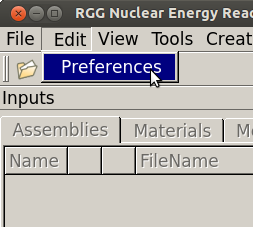
\includegraphics[width=0.5\linewidth]{Images/mesh-1.png}
		\caption{Opening RGG preferences.}
		\label{fig:Mesh1}
	\end{center}
\end{figure}

This should bring up the System Preferences window.  To add AssyGen, CoreGen, or Cubit, click Browse to locate the executable and press Open to get back to the System Preferences window.

\begin{figure}[H]
	\begin{center}
		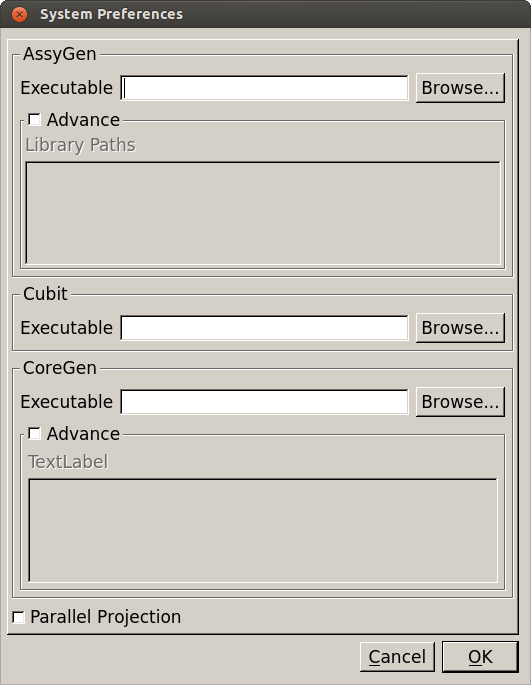
\includegraphics[width=0.5\linewidth]{Images/mesh-2.png}
		\caption{The preferences window.}
		\label{fig:Mesh2}
	\end{center}
\end{figure}

\section{Generating a Mesh from an INP file}

After opening an INP file and setting up your preferences to include the paths to AssyGen, CoreGen, and Cubit, you can generate a mesh though a dialog accessed through the Tools menu.  Note the X icon for the assemblies and core in the inputs pane.  This designates that RGG believes that these components need to be meshed.

\begin{figure}[H]
	\begin{center}
		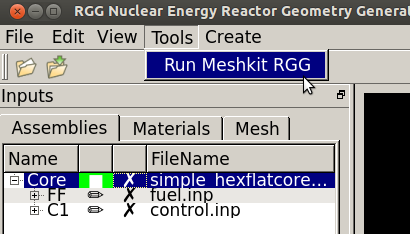
\includegraphics[width=0.5\linewidth]{Images/mesh-3.png}
		\caption{Opening the Run MeshKit RGG dialog.}
		\label{fig:Mesh3}
	\end{center}
\end{figure}

You may be prompted to save changes before proceeding.

The dialog should be populated with the assemblies that need to be re-meshed automatically.  In the example below, two assemblies need to be meshed, which also means that the core must be remeshed.

\begin{figure}[H]
	\begin{center}
		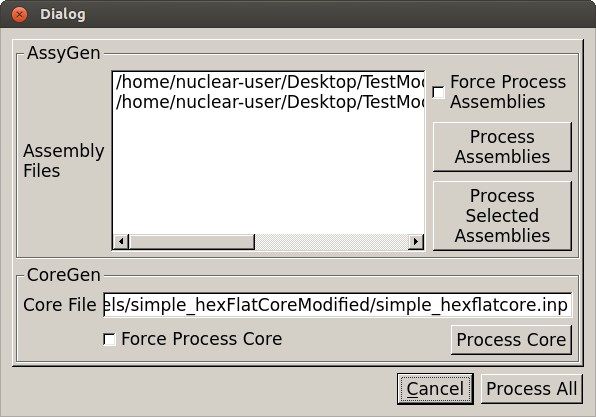
\includegraphics[width=0.5\linewidth]{Images/mesh-4.png}
		\caption{The Run MeshKit RGG dialog.}
		\label{fig:Mesh4}
	\end{center}
\end{figure}

Note that you can force the meshing of any assembly, or selectively mesh only certain assemblies with the Force Process Assemblies checkbox and the Process Selected Assemblies button.  The same applies for the core too with the Force Process Core checkbox.  We'll click the Process All button without changing any defaults to process the assemblies that need to be meshed and then process the core.  A window that gives you the status of the processing should come up, similar to the one below:

\begin{figure}[H]
	\begin{center}
		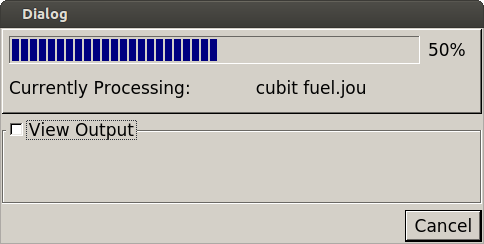
\includegraphics[width=0.5\linewidth]{Images/mesh-5.png}
		\caption{Running meshing.}
		\label{fig:Mesh5}
	\end{center}
\end{figure}

You can see the output of MeshKit's AssyGen and CoreGen by clicking on the View Output checkbox.

To verify that the assemblies and core have been meshed, note that the X icons seen previously should now be green squares, as shown in ~\ref{fig:Mesh6}.

\begin{figure}[H]
	\begin{center}
		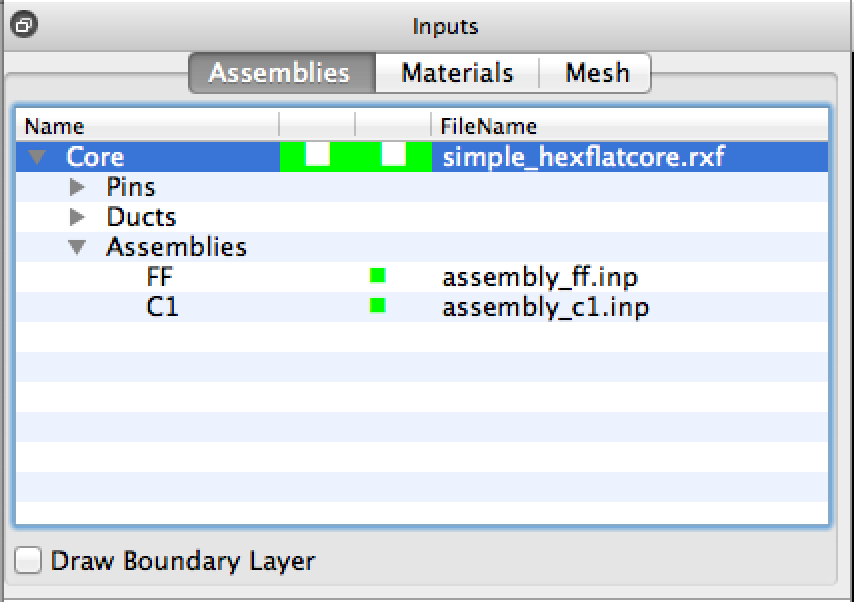
\includegraphics[width=0.5\linewidth]{Images/mesh-6.png}
		\caption{Verifying successful meshing.}
		\label{fig:Mesh6}
	\end{center}
\end{figure}

Note that the mesh needs to be loaded in after MeshKit creates it.  During this process, the Tools menu is inaccessible.